\achapter{26}{Least Squares Approximations} \label{sec:least_squares}

\vspace*{-17 pt}
\framebox{
\parbox{\dimexpr\linewidth-3\fboxsep-3\fboxrule}
{\begin{fqs}
\item How, in general, can we find a least squares approximation to a system $A \vx = \vb$?
\item If the columns of $A$ are linearly independent, how can we find a least squares approximation to $A \vx = \vb$ using just matrix operations?
\item Why are these approximations called ``least squares" approximations?  
\end{fqs}}}% \hspace*{3 pt}}

\vspace*{13 pt}

\csection{Application: Fitting Functions to Data}

Data is all around us. Data is collected on almost everything and it is important to be able to use data to make predictions. However, data is rarely well-behaved and so we generally need to use approximation techniques to estimate from the data. One technique for this is least squares approximations. As we will see, we can use linear algebra to fit a variety of different types of curves to data. 


\csection{Introduction}

In this section our focus is on fitting linear and polynomial functions to data sets. 

\begin{pa} \label{pa:LS_1} NBC was awarded the U.S. television broadcast rights to the 2016 and 2020 summer Olympic games. Table \ref{T:LS_Olympics} lists the amounts paid (in millions of dollars) by NBC sports for the 2008 through 2012 summer Olympics plus the recently concluded bidding for the 2016 and 2020 Olympics, where year 0 is the year 2008. (We will assume a simple model here, ignoring variations such as value of money due to inflation, viewership data which might affect NBC's expected revenue, etc.) Figure \ref{F:LS_Olympics} shows a plot of the data. Our goal in this activity is to find a linear function $f$ defined by $f(x) = a_0 + a_1x$ that fits the data well. 

\begin{minipage}{\textwidth}
  \begin{minipage}[b]{0.49\textwidth}
    \centering
    \renewcommand{\arraystretch}{1.2}
\begin{tabular}{|c|c|} \hline
Year    &Amount \\ \hline
0	&894   \\ \hline 
4	&1180  \\ \hline 
8	&1226  \\ \hline 
12	&1418\\ \hline
\end{tabular}
      \captionof{table}{Olympics television broadcast rights.}
      \label{T:LS_Olympics}
      \hfill
    \end{minipage}
  \begin{minipage}[b]{0.49\textwidth}
    \centering
    \resizebox{!}{1.35in}{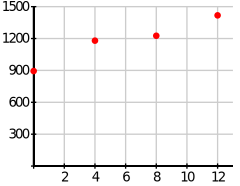
\includegraphics{7_d_pa_3}}
    \captionof{figure}{A plot of the data.}
    \label{F:LS_Olympics}
  \end{minipage}
 
\end{minipage}

If the data were actually linear, then the data would satisfy the system
\begin{alignat*}{4}
{}a_0 &{}+{}	&{0}a_1 &= &894&{}  \\
{}a_0 &{}+{}	&{4}a_1 &= &1180&{}  \\
{}a_0 &{}+{}	&{8}a_1 &= &1226&{}  \\
{}a_0 &{}+{}	&{12}a_1 &= &1418&{.}
\end{alignat*}
The vector form of this equation is
\[a_0 [1 \ 1 \ 1 \ 1]^{\tr} + a_1[0 \ 4 \ 8 \ 12]^{\tr} = [894 \ 1180 \ 1226 \ 1418]^{\tr}.\]
This equation does not have a solution, so we seek the best approximation to a solution we can find.  That is, we want to find $a_0$ and $a_1$ so that the line $f(x) = a_0+a_1x$ provides a best fit to the data.  

Letting $\vv_1 = [1 \ 1 \ 1 \ 1]^{\tr}$ and $\vv_2 = [0 \ 4 \ 8 \ 12]^{\tr}$, and $\vb = [894 \ 1180 \ 1226 \ 1418]^{\tr}$, our vector equation becomes
\[a_0 \vv_1 + a_1\vv_2 = \vb.\]
To make a best fit, we will minimize the square of the distance between $\vb$ and a vector of the form $a_0\vv_1 + a_1 \vv_2$. That is, minimize
\begin{equation} \label{eq:LS_line_1} 
||\vb - (a_0 \vv_1 + a_1\vv_2)||^2.
\end{equation} 
Rephrasing this in terms of projections, we are looking for the vector in $W = \Span\{\vv_1, \vv_2\}$ that is closest to $\vb$.  In other words, the values of $a_0$ and $a_1$ will occur as the weights when we write $\proj_{W} \vb$ as a linear combination of $\vv_1$ and $\vv_2$. The one wrinkle in this problem is that we need an orthogonal basis for $W$ to find this projection. Use appropriate technology throughout this activity. 

\be
\item Find an orthogonal basis $\CB = \{\vw_1, \vw_2\}$ for $W$. 

\item Use the basis $\CB$ to find $\vy = \proj_{W} \vb$ as illustrated in Figure \ref{F:6_f_proj}.
\begin{figure}[h]
    \begin{center}
    \resizebox{!}{1.45in}{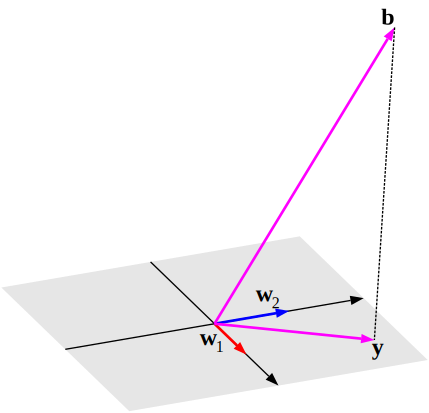
\includegraphics{6_f_O_proj}}
    \caption{Projecting $\vb$ onto $W$.}
    \label{F:6_f_proj}
    \end{center}
    \end{figure} 

\item Find the values of $a_0$ and $a_1$ that give our best fit line by writing $\vy$ as a linear combination of $\vv_1$ and $\vv_2$. 

\item Draw a picture of your line from the previous part on the axes with the data set. How well do you think your line approximates the data? Explain. 
	
\ee

\end{pa}

 \csection{Least Squares Approximations}
 
In Section \ref{sec:gram_schmidt} we saw that the projection of a vector $\vv$ in $\R^n$ onto a subspace $W$ of $\R^n$ is the best approximation to $\vv$ of all the vectors in $W$. In fact, if $\vv = [v_1 \ v_2 \ \ldots \ v_n]^{\tr}$ and $\proj_W \vv =  [w_1 \ w_2 \ w_3 \ \ldots \ w_m]^{\tr}$, then the error in approximating $\vv$ by $\vw$ is given by 
\[|| \vv - \proj_W \vv ||^2 = \sum_{i=1}^m (v_i - w_i)^2.\]
In the context of Preview Activity \ref{pa:LS_1}, we projected the vector $\vb$ onto the span of the vectors $\vv_1 = [1 \ 1 \ 1 \ 1]^{\tr}$ and $\vv_2 = [0 \ 4 \ 8 \ 12]^{\tr}$. The projection minimizes the distance between the vectors in $W$ and the vector $\vb$ (as shown in Figure \ref{F:6_f_proj}), and also produces a line which minimizes the sums of the squares of the vertical distances from the line to the data set as illustrated in Figure \ref{F:LS_Olympics2} with the olympics data. This is why these approximations are called least squares approximations. 

\begin{figure}[h]
\begin{center}
\resizebox{!}{2.0in}{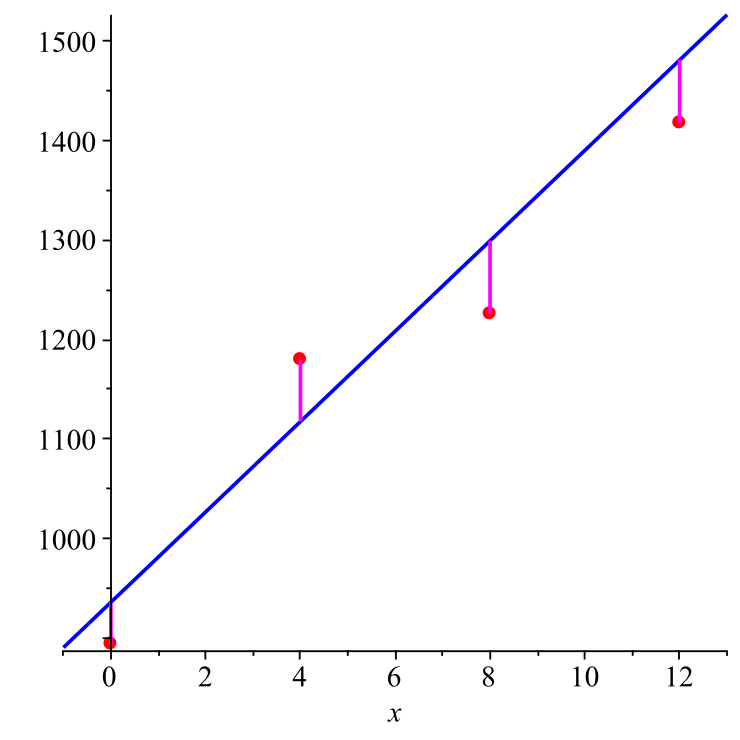
\includegraphics{Regression1}}
\caption{Least squares linear approximation}
\label{F:LS_Olympics2}
\end{center}
\end{figure}

While we can always solve least squares problems using projections, we can often avoid having to create an orthogonal basis when fitting functions to data. We work in a more general setting, showing how to fit a polynomial of degree $n$ to a set of data points. Our goal is to fit a polynomial $p(x) = a_0+a_1x+a_2x^2+ \cdots + 
a_nx^n$ of degree $n$ to $m$ data points $(x_1,y_1)$, $(x_2,y_2)$, $\ldots$, $(x_m,y_m)$, no two of which have the same $x$ coordinate. In the unlikely event that the polynomial $p(x)$ actually passes through the $m$ points, then we would have the $m$ equations
\begin{alignat*}{7}
y_1 &{}={} &{a_0} &{}+{} &{a_1}x_1 &{}+{} &{a_2}x_1^2 &{}+{} &\cdots &{}+{} &{a_{n-1}}x_1^{n-1} &{}+{} &{a_n}x_1^n  \\
y_2 &{}={} &{a_0} &{}+{} &{a_1}x_2 &{}+{} &{a_2}x_2^2 &{}+{} &\cdots &{}+{} &{a_{n-1}}x_2^{n-1} &{}+{} &{a_n}x_2^n  \\
y_3 &{}={} &{a_0} &{}+{} &{a_1}x_3 &{}+{} &{a_2}x_3^2 &{}+{} &\cdots &{}+{} &{a_{n-1}}x_3^{n-1} &{}+{} &{a_n}x_3^n  \\
{}   &{}     &{}       &{}      &{}          &{}      &{}             &{}       &\vdots &{}     &{}                            &{}       &{}            \\
y_m &{}={} &{a_0} &{}+{} &{a_1}x_m &{}+{} &{a_2}x_m^2 &{}+{} &\cdots &{}+{} &{a_{n-1}}x_m^{n-1} &{}+{} &{a_n}x_m^n
\end{alignat*}
in the $n+1$ unknowns $a_0$, $a_1$, $\ldots$, $a_{n-1}$, and $a_n$.

The $m$ data points are known in this situation and the coefficients $a_0$, $a_1$, $\ldots$, $a_n$ are the unknowns. To write the system in matrix-vector form, the coefficient matrix $M$ is
\[M = \left[ \begin{array}{cccccc} 1&x_1&x_1^2& \cdots &x_1^{n-1}&x_1^{n} \\ 1&x_2&x_2^2& \cdots &x_2^{n-1}&x_2^{n} \\ 1&x_3&x_3^2& \cdots &x_3^{n-1}&x_3^{n} \\ \vdots & \vdots & \vdots & \cdots &\vdots &\vdots \\ 1&x_m&x_m^2& \cdots &x_m^{n-1}&x_m^{n} \end{array} \right],\]
while the vectors $\va$ and $\vy$ are
\[\va = \left[ \begin{array}{c} a_{0} \\ a_{1} \\ a_{2} \\ \vdots \\ a_{n-1} \\a_{n} \end{array} \right] \text{ and } \vy = \left[ \begin{array}{c} y_{1} \\ y_{2} \\ y_{3} \\ \vdots \\ y_{m-1} \\ y_{m} \end{array} \right].\]
Letting $\vy = [y_1 \ y_2 \ \ldots \ y_m]^{\tr}$ and $\vv_i = [x_1^{i-1} \ x_2^{i-1} \ \ldots \ x_m^{i-1}]^{\tr}$ for $1 \leq i \leq n+1$, the vector form of the system is 
\[\vy = a_0\vv_1 + a_1 \vv_2 +  \cdots + a_n \vv_{n+1}.\]

Of course, it is unlikely that the $m$ data points already lie on a polynomial of degree $n$, so the system will usually have no solution. So instead of attempting to find coefficients $a_0$, $a_1$, $\ldots$, $a_n$ that give a solution to this system, which may be impossible, we instead look for a vector that is ``close" to a solution. As we have seen, the vector $\proj_{W} \vy$, where $W$ is the span of the columns of $M$, minimizes the sum of the squares of the differences of the components. That is, our desired approximation to a solution to $M \vx = \vy$ is the projection of $\vy$ onto $\Col M$. Now $\proj_W \vy$ is a linear combination of the columns of $M$, so $\proj_W \vy = M \va^*$ for some vector $\va^*$. This vector $\va^*$ then minimizes $|| \proj_{\perp W} \vy|| = ||\vy - M \va ||$. That is, if we let $(M\va)^{\tr} = [b_1 \ b_2 \ b_3 \ \cdots \ b_m]$, we are minimizing 
\begin{equation*}
||\vy - M\va||^2 = (y_1-b_1)^2 + (t_2-b_2)^2 + \cdots + (y_m-b_m)^2. \label{eq:ls_1}
\end{equation*}
The expression $||\vy - M\va||^2$ measures the error in our approximation. 

The question we want to  answer is how we can find the vector $\va^*$ that minimizes $||\vy -M\va||$ in a way that is more convenient than computing a projection. We answer this question in a general setting in the next activity. 

\begin{activity} \label{act:LS_matrices} Let $A$ be an $m \times n$ matrix and let $\vb$ be in $\R^m$. Let $W = \Col A$. Then $\proj_W \vb$ is in $\Col A$, so let $\vx^*$ be in $\R^{n}$ such that $A\vx^* = \proj_W \vb$. 
	\ba
    \item Explain why $\vb - A\vx^*$ is orthogonal to every vector of the form $A\vx$, for any $\vx$ in $\R^{n}$. That is, $\vb - A\vx^*$ is orthogonal to $\Col A$. 

    \item Let $\va_i$ be the $i$th column of $A$. Explain why $\va_i \cdot \left(\vb - A\vx^*\right) = 0$. From this, explain why $A^{\tr}\left(\vb - A\vx^*\right) = 0$. 
    
    \item From the previous part, show that $\vx^*$ satisfies the equation
\[A^{\tr}A\vx^* = A^{\tr}\vb.\]
%    From this we can conclude that if $A^{\tr}A$ is invertible, then
%\[\vx^* = \left(A^{\tr}A\right)^{-1}A^{\tr}\vb.\]


    \ea
    
\end{activity}


The result of Activity \ref{act:LS_matrices} is that we can now do least squares polynomial approximations with just matrix operations. We summarize this in the following theorem.

\begin{theorem} \label{thm:6_f_least_squares_1} The least squares solutions to the system $A \vx = \vb$ are the solutions to the corresponding system 
    \begin{equation} \label{eq:6_f_normal_equations}
    A^{\tr}A\vx = A^{\tr}\vb.
    \end{equation}
\end{theorem}

The equations in the system (\ref{eq:6_f_normal_equations}) are called the \emph{normal equations} for $A \vx = \vb$. To illustrate, with the Olympics data, our data points are $(0, 894)$, $(4, 1180)$, $(8, 1226)$, $(12,1418)$ with $\vy = [894 \ 1180 \ 1226 \ 1418]^{\tr}$. So $M = \left[ \begin{array}{cc} 1&0 \\ 1&4 \\ 1&8 \\ 1&12 \end{array} \right]$. Notice that $M^{\tr}M$ is invertible, to find the degree 1 approximation to the data, technology shows that 
\[\va^* = \left(M^{\tr}M\right)^{-1}M^{\tr}\vy = \left[ \frac{4684}{5} \ \frac{809}{20}\right]\]
just as in Preview Activity \ref{pa:LS_1}. 


\begin{activity} Now use the least squares method to find the best polynomial approximations (in the least squares sense) of degrees 2 and 3 for the Olympics data set in Table \ref{T:LS_Olympics}. Which polynomial seems to give the ``best" fit? Explain why. Include a discussion of the errors in your approximations. Use your ``best" least squares approximation to estimate how much NBC might pay for the television rights to the 2024 Olympic games. Use technology as appropriate.

\end{activity}

The solution with our Olympics data gave us the situation where $M^{\tr}M$ was invertible. This corresponded to a unique least squares solution $ \left(M^{\tr}M\right)^{-1}M^{\tr}\vy$. It is reasonable to ask when this happens in general. To conclude this section, we will demonstrate that if the columns of a matrix $A$ are linearly independent, then $A^{\tr}A$ is invertible.

\begin{activity} \label{act:LS_invertible} Let $A$ be an $m \times n$ matrix with linearly independent columns.
\ba
\item What must be the relationship between $m$ and $n$? Explain. 

\item We know that an $n \times n$ matrix $M$ is invertible if and only if the only solution to the homogeneous system $M \vx = \vzero$ is $\vx = \vzero$. Note that $A^{\tr}A$ is an $n \times n$ matrix. Suppose that $A^{\tr}A \vx = \vzero$ for some $\vx$ in $\R^n$. 
	\begin{enumerate}[i.]
	\item Show that $||A\vx|| = 0$. (Hint: What is $\vx^{\tr} (A^{\tr}A \vx)$?)

	\item What does $||A\vx|| = 0$ tell us about $\vx$ in relation to $\Nul A$? Why?

	\item What is $\Nul A$? Why? What does this tell us about $\vx$ and then about $A^{\tr}A$?
	

	\end{enumerate}

\ea

\end{activity}

We summarize the result of Activity \ref{act:LS_invertible} in the following theorem.

\begin{theorem} \label{thm:6_f_least_squares_2} If the columns of $A$ are linearly independent, then the least squares solution $\vx^*$ to the system $A \vx = \vb$ is
\[\vx^* = \left(A^{\tr}A\right)^{-1}A^{\tr}\vb.\]
\end{theorem}

If the columns of $A$ are linearly dependent, we can still solve the normal equations, but will obtain more than one solution. In a later section we will see that we can also use a pseudoinverse in these situations. 

\csection{Examples}

\ExampleIntro

\begin{example} According to the Centers for Disease Control and Prevention\footnote{ \url{https://www.cdc.gov/growthcharts/html_charts/lenageinf.htm}}, the average length of a male infant (in centimeters) in the US as it ages (with time in months from 1.5 to 8.5) is given in Table \ref{T:lengths}. 
\begin{table}[h]
\begin{center}
\begin{tabular}{|c||c|c|c|c|c|c|c|c|} \hline
Age (months)	&1.5	&2.5	&3.5	&4.5	&5.5	&6.5	&7.5	&8.5 \\ \hline
Average Length (cm)	&56.6&59.6&62.1&64.2&66.1&67.9&69.5&70.9 \\ \hline
\end{tabular}
\caption{Average lengths of male infants.}
\label{T:lengths}
\end{center}
\end{table}
In this problem we will find the line and the quadratic of best fit in the least squares sense to this data. We treat age in months as the independent variable and length in centimeters as the dependent variable. 
	\ba
	\item Find a line that is the best fit to the data in the least squares sense. Draw a picture of your least squares solution against a scatterplot of the data. 

%	\item Even though the data is not perfectly linear, let us assume for a moment that a line of the form $f(x) = a_1x+a_0$ contains all of the data points. 
%		\begin{enumerate}[i.]
%		\item Write a matrix equation of the form $A \vx = \vb$ that represents the data.

%		\item Find the best least squares solution to the system $A \vx = \vb$. Use appropriate technology to perform any matrix operations. Draw a picture of your least squares solution against a scatterplot of the data. 

%		\end{enumerate}
		
	\item Now find the least squares quadratic of the form $q(x) = a_2x^2+a_1x+a_0$ to the data. Draw a picture of your least squares solution against a scatterplot of the data. 

	
	\ea
	


\ExampleSolution

	\ba
	\item We assume that a line of the form $f(x) = a_1x+a_0$ contains all of the data points.  The first data point would satisfy $1.5a_1+a_0 = 56.6$, the second $2.5a_1+a_0 = 59.6$, and so on, giving us the linear system
\begin{alignat*}{3}
{1.5}a_1	&{}+{}	&a_0 &{}={} 56.6{} \\ 
{2.5}a_1	&{}+{}	&a_0 &{}={} 59.6{} \\
{3.5}a_1	&{}+{}	&a_0 &{}={} 62.1{} \\
{4.5}a_1	&{}+{}	&a_0 &{}={} 64.2{}  \\
{5.5}a_1	&{}+{}	&a_0 &{}={} 66.1{} \\
{6.5}a_1	&{}+{}	&a_0 &{}={} 67.9{} \\
{7.5}a_1	&{}+{}	&a_0 &{}={} 69.5{} \\
{8.5}a_1	&{}+{}	&a_0 &{}={} 70.9{.}
\end{alignat*}
Letting 
\[A = \left[ \begin{array}{cc} 1.5&1 \\ 2.5&1 \\ 3.5&1 \\ 4.5&1 \\ 5.5&1 \\ 6.5&1 \\ 7.5&1 \\ 8.5&1 \end{array} \right], \ \vx = \left[ \begin{array}{c} a_1\\a_0 \end{array} \right], \ \text{ and } \ \vb=\left[ \begin{array}{c} 56.6\\59.6\\62.1\\64.2\\66.1\\67.9\\69.5\\70.9 \end{array} \right],\]
we can write this system in the matrix form  $A \vx = \vb$. Neither column of $A$ is a multiple of the other, so the columns of $A$ are linearly independent. The least squares solution $\vx^*$ to the system is then found by 
\[\vx^* = \left(A^{\tr}A\right)^{-1}A^{\tr} \vb.\]
Technology shows that (with entries rounded to 3 decimal places), $\left(A^{\tr}A\right)^{-1}A^{\tr}$ is 
\[ \left[\arraycolsep=2.5pt \begin{array}{rrrrcrrr} - 0.083&- 0.060&- 0.036&- 0.012& 0.012& 0.036& 0.060& 0.083\\ 0.542& 0.423& 0.304& 0.185& 0.065&- 0.054&- 0.173&- 0.292 \end{array} \right],\]
and 
\[\vx^* \approx \left[ \begin{array}{cc} 2.011 \\ 54.559 \end{array} \right].\]
So the least squares linear function to the data is $f(x) \approx 2.011x + 54.559$. A graph of $f$ against the data points is shown at left in Figure \ref{F:LS_linear}. 
\begin{figure}[h]
\begin{center}
\resizebox{!}{2.0in}{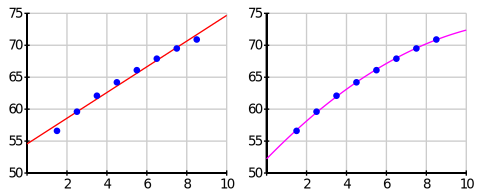
\includegraphics{7_d_least_squares_line}} 
%\resizebox{!}{1.5in}{\includegraphics{least_squares_line}} \hspace{0.2in} \resizebox{!}{1.5in}{\includegraphics{least_squares_quadratic}}
\end{center}
\caption{Left: Least squares line. Right: Least squares quadratic.}
\label{F:LS_linear}
\end{figure}   
		
	\item The first data point would satisfy $(1.5^2)a_2+1.5a_1+a_0 = 56.6$, the second $(2.5)^2a_2+2.5a_1+a_0 = 59.6$, and so on, giving us the linear system
\begin{alignat*}{4}
{1.5^2}a_2	&{}+{}	&{1.5}a_1	&{}+{}	&a_0 &{}={} 56.6{} \\ 
{2.5^2}a_2	&{}+{}	&{2.5}a_1	&{}+{}	&a_0 &{}={} 59.6{} \\
{3.5^2}a_2	&{}+{}	&{3.5}a_1	&{}+{}	&a_0 &{}={} 62.1{} \\
{4.5^2}a_2	&{}+{}	&{4.5}a_1	&{}+{}	&a_0 &{}={} 64.2{}  \\
{5.5^2}a_2	&{}+{}	&{5.5}a_1	&{}+{}	&a_0 &{}={} 66.1{} \\
{6.5^2}a_2	&{}+{}	&{6.5}a_1	&{}+{}	&a_0 &{}={} 67.9{} \\
{7.5^2}a_2	&{}+{}	&{7.5}a_1	&{}+{}	&a_0 &{}={} 69.5{} \\
{8.5^2}a_2	&{}+{}	&{8.5}a_1	&{}+{}	&a_0 &{}={} 70.9{.}
\end{alignat*}
Letting 
\[A = \left[ \begin{array}{ccc} 1.5^2&1.5&1 \\ 2.5^2&2.5&1 \\ 3.5^2&3.5&1 \\ 4.5^2&4.5&1 \\ 5.5^2&5.5&1 \\ 6.5^2&6.5&1 \\ 7.5^2&7.5&1 \\ 8.5^2&8.5&1 \end{array} \right], \ \vx = \left[ \begin{array}{c} a_2\\a_1\\a_0 \end{array} \right], \ \text{ and } \ \vb=\left[ \begin{array}{c} 56.6\\59.6\\62.1\\64.2\\66.1\\67.9\\69.5\\70.9 \end{array} \right],\]
we can write this system in the matrix form  $A \vx = \vb$. 

Technology shows that every column of the reduced row echelon form of $A$ contains a pivot, so the columns of $A$ are linearly independent. The least squares solution $\vx^*$ to the system is then found by 
\[\vx^* = \left(A^{\tr}A\right)^{-1}A^{\tr} \vb.\]
Technology shows that (with entries rounded to 3 decimal places) $\left(A^{\tr}A\right)^{-1}$ is 
\[\left[ \arraycolsep=2.5pt  \begin{array}{rrrrrrrr}  0.042& 0.006&- 0.018&- 0.030&- 0.030&- 0.018& 0.006& 0.042\\ - 0.500&- 0.119& 0.143& 0.286& 0.310& 0.214& 0.000&-0.333\\  1.365& 0.540&- 0.049&- 0.403&-0.522&- 0.406&- 0.055& 0.531\end {array} \right],\]
and 
\[\vx^* \approx \left[ \begin{array}{r} -0.118 \\ 3.195 \\ 52.219 \end{array} \right].\]
So the least squares quadratic function to the data is $q$ defined by $q(x) \approx -0.118x^2+3.195x + 52.219$. A graph of $q$ against the data points is shown at right in Figure \ref{F:LS_linear}. 
 	
	\ea

\end{example}

\begin{example} Least squares solutions can be found through a QR factorization, as we explore in this example. Let $A$ be an $m \times n$ matrix with linearly independent columns and QR factorization $A = QR$. Suppose that $\vb$ is not in $\Col A$ so that the system $A \vx = \vb$ is inconsistent. We know that the least squares solution $\vx^*$ to $A \vx = \vb$ is 
\begin{equation} \label{eq:ls_example}
\vx^* = \left(A^{\tr}A\right)^{-1}A^{\tr}\vb.
\end{equation}
\ba
\item Replace $A$ by its QR factorization in (\ref{eq:ls_example}) to show that 
\[\vx^* = R^{-1}Q^{\tr} \vb.\]
(Hint: Use the fact that $Q$ is orthogonal and $R$ is invertible.)

\item Consider the data set in Table \ref{T:life_exectancy}, which shows the average life expectance in years in the US for selected years from 1950 to 2010. 
\begin{table}[ht]
\begin{center}
\begin{tabular}{l|cccccc}
year	&1950 	&1965 	&1980 	&1995 	&2010 \\
age	&68.14	&70.21	&73.70	&75.98	&78.49 
\end{tabular}
\caption{Life expectancy in the US.}
\label{T:life_exectancy}
\end{center}
\end{table}
(Data from macrotrends at \url{https://www.macrotrends.net/countries/USA/united-states/life-expectancy}.) 
	\begin{enumerate}[i.]
	\item Use (\ref{eq:ls_example}) to find the least squares linear fit to the data set. 
	
	\item Use appropriate technology to find the QR factorization of an appropriate matrix $A$, and use the QR decomposition to find the least squares linear fit to the data. Compare to what you found in part i. 

	\end{enumerate}
	
\ea

\end{example}

\ExampleSolution
\ba
\item Replacing $A$ with $QR$ and using the fact that $R$ is invertible and $Q$ is orthogonal to see that 
\begin{align*}
\vx^* &= \left(A^{\tr}A\right)^{-1}A^{\tr}\vb \\
	 &= \left((QR)^{\tr}QR\right)^{-1} (QR)^{\tr} \vb \\
	&= \left(R^{\tr}Q^{\tr}QR\right) R^{\tr}Q^{\tr} \vb \\
	&= \left(R^{\tr}R\right)^{-1}R^{\tr}Q^{\tr} \vb \\
	&= R^{-1}\left(R^{\tr}\right)^{-1}R^{\tr} Q^{\tr} \vb \\
	&= R^{-1}Q^{\tr} \vb.
\end{align*}
So if $A = QR$ is a QR factorization of $A$, then the least squares solution to $A \vx = \vb$ is $R^{-1}Q^{\tr} \vb$. 

\item 
	\begin{enumerate}[i.]
	\item A linear fit to the data will be provided by the least squares solution to $A \vx = \vb$, where 
\[A = \left[ \begin{array}{cc} 1&1950 \\ 1&1965 \\ 1 &1980 \\  1&1995 \\ 1 &2010 \end{array} \right], \ \vx = \left[ \begin{array}{c} a\\b \end{array} \right], \ \text{ and } \ \vb =  \left[ \begin{array}{c} 68.14\\70.21\\73.70\\75.98	\\78.49 \end{array} \right].\]
Technology shows that 
\[\left(A^{\tr}A\right)^{-1}A^{\tr} \vb \approx [-276.1000 \ 0.1765]^{\tr}.\]
	
	\item Technology shows that $A = QR$, where 
\[Q = \left[\renewcommand{\arraystretch}{1.4}  \begin{array}{cr} \frac{1}{\sqrt{5}}&-\frac{2}{\sqrt{10}} \\ \frac{1}{\sqrt{5}}&-\frac{1}{\sqrt{10}} \\ \frac{1}{\sqrt{5}}&0 \\ \frac{1}{\sqrt{5}}&\frac{1}{\sqrt{10}} \\ \frac{1}{\sqrt{5}}&\frac{2}{\sqrt{10}} \end{array} \right] \text{ and } R = \left[ \begin{array}{cc} \sqrt{5}&1980 \sqrt{5} \\ 0&15 \sqrt{10} \end{array} \right].\]
Then we have that 
\[R^{-1} Q^{\tr} \vb \approx [-276.1000 \ 0.1765]^{\tr},\]
just as in part i. 	

	\end{enumerate}
	
\ea

\csection{Summary}
\begin{itemize}
\item A least squares approximation to $A \vx = \vb$ is found by orthogonally projecting $\vb$ onto $\Col A$. 
\item If the columns of $A$ are linearly independent, then the least squares approximation to $A \vx = \vb$ is $\left(A^{\tr}A\right)^{-1}A^{\tr} \vb$. 
\item The least squares solution to $A \vx = \vb$, where $A\vx = [y_1 \ y_2 \ \ldots \ y_m]$ and $\vb = [b_1 \ b_2 \ \ldots \ b_ m]^{\tr}$, minimizes the distance $||A\vx - \vb||$, where 
\begin{equation*}
||A\vx - \vb||^2 = (y_1-b_1)^2 + (y_2-b_2)^2 + \cdots + (y_m-b_m)^2. 
\end{equation*}
So the least squares solution minimizes a sum of squares. 
 
\end{itemize}


\csection{Exercises}

\be
\item The University of Denver Infant Study Center investigated whether babies take longer to learn to crawl in cold months, when they are often bundled in clothes that restrict their movement, than in warmer months. The study sought a relationship between babies' first crawling age and the average temperature during the month they first try to crawl (about 6 months after birth). Some of the data from the study is in Table \ref{T:7_d_infants}. Let $x$ represent the temperature in degrees Fahrenheit and $C(x)$ the average crawling age in months. 

\begin{table}[ht]
\begin{center}
\begin{tabular}{|l||c|c|c|c|} \hline
$x$		&33		&37		&48		&57 \\ \hline
$C(x)$	&33.83	&33.35	&33.38	&32.32 \\ \hline
\end{tabular}
\end{center}
\caption{Crawling age.}
\label{T:7_d_infants}
\end{table}
	\ba
	\item Find the least squares line to fit this data. Plot the data and your line on the same set of axes. (We aren't concerned about whether a linear fit is really a good choice outside of this data set, we just fit a line to it to see what happens.)
	
	\item Use your least squares line to predict the average crawling age when the temperature is 65. 
	\ea


\item The cost, in cents, of a first class postage stamp in years from 1981 to 1995 is shown in Table \ref{T:7_d_stamps}.

	\ba
	\item Find the least squares line to fit this data. Plot the data and your line on the same set of axes. 
	\item Now find the least squares quadratic approximation to this data. Plot the quadratic function on same axes as your linear function. 
	\item Use your least squares line and quadratic to predict the cost of a postage stamp in this year. Look up the cost of a stamp today and determine how accurate your prediction is. Which function gives a better approximation? Provide reasons for any discrepancies.  
	\ea

\begin{table}[h]
\begin{center}
\begin{tabular}{|l||c|c|c|c|c|} \hline
Year	&1981	&1985	&1988	&1991	&1995 \\ \hline
Cost	&20		&22		&25		&29		&32  \\ \hline
\end{tabular}
\end{center}
\caption{Cost of postage.}
\label{T:7_d_stamps}
\end{table}


\item According to \emph{The Song of Insects} by G.W. Pierce (Harvard College Press, 1948) the sound of striped ground crickets chirping, in number of chirps per second, is related to the temperature. So the number of chirps per second could be a predictor of temperature. The data Pierce collected is shown in the table and scatterplot below, where $x$ is the (average) number of chirps per second and $y$ is the temperature in degrees Fahrenheit. 

\begin{center}
\begin{minipage}{2in}
\begin{center}
\begin{tabular}{|c|c|} \hline
$x$	&$y$ \\ \hline
20.0	&88.6 \\ \hline
16.0	&71.6 \\ \hline
19.8	&93.3 \\ \hline
18.4	&84.3 \\ \hline
17.1	&80.6 \\ \hline
15.5	&75.2 \\ \hline
14.7	&69.7 \\ \hline
17.1	&82.0 \\ \hline
15.4	&69.4 \\ \hline
16.2	&83.3 \\ \hline
15.0	&79.6 \\ \hline
17.2	&82.6 \\ \hline
16.0	&80.6 \\ \hline
17.0	&83.5 \\ \hline
14.4	&76.3 \\ \hline
\end{tabular}
\end{center} 
\end{minipage} \hspace{0.2in}
\begin{minipage}{2.5in}
 \begin{center}
      \resizebox{2.55in}{!}{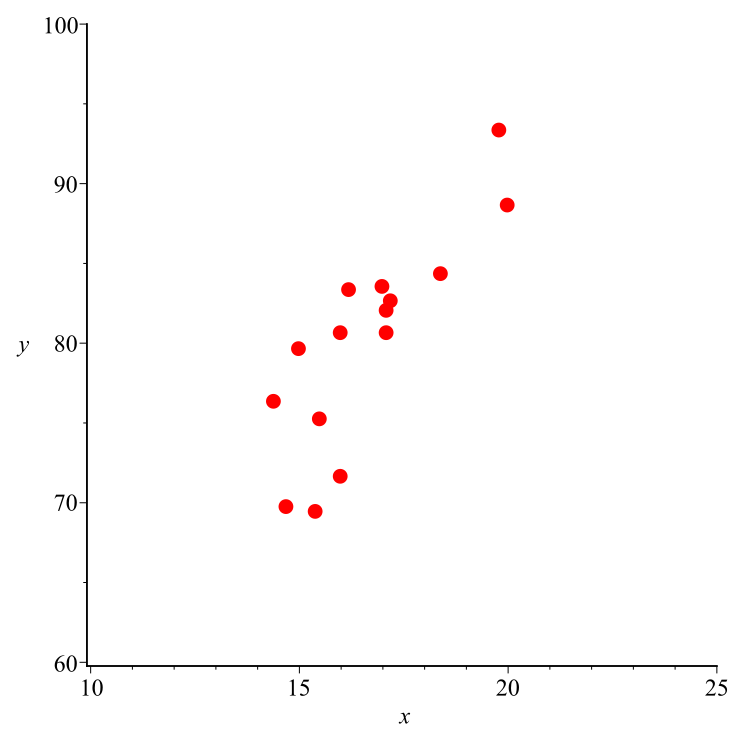
\includegraphics{10_7_crickets.eps}}
    \end{center}
    \end{minipage}
    \end{center}
The relationship between $x$ and $y$ is not exactly linear, but looks to have a linear pattern. It could be that the relationship is really linear but experimental error causes the data to be slightly inaccurate. Or perhaps the data is not linear, but only approximately linear. Find the least squares linear approximation to the data. 

\item We showed that if the columns of $A$ are linearly independent, then $A^{\tr}A$ is invertible. Show that the reverse implication is also true. That is, show that if $A^{\tr}A$ is invertible, then the columns of $A$ are linearly independent.

%\item Let $\vv$ be a vector in $\R^k$. Suppose that  $\vv\cdot \vw= 0$ for every vector $\vw$ in $\R^k$. Show that $\vv= \vzero$.
	

\item \label{ex:6_f_not_li} Consider the small data set of points $S = \{(2,1), (2,2), (2,3)\}$. 
\ba 
\item Find a linear system $A \vx = \vb$ whose solution would define a least squares linear approximation to the data in set $S$.

\item Explain what happens when we attempt to find the least squares solution $\vx^*$ using the matrix $\left(A^{\tr}A\right)^{-1}A^{\tr}$. Why does this happen?

\item Does the system $A \vx = \vb$ have a least squares solution? If so, how many and what are they? If not, why not?

\item Fit a linear function of the form $x = a_0 + a_1y$ to the data. Why should you have expected the answer?  

\ea

\item \label{ex:6_f_ranks} Let $M$ and $N$ be any matrices such that $MN$ is defined. In this exercise we investigate relationships between ranks of various matrices. 
\ba
\item Show that $\Col MN$ is a subspace of $\Col M$. Use this result to explain why $\rank(MN) \leq \rank(M)$. 

\item Show that $\rank\left(M^{\tr}M\right) = \rank(M) = \rank\left(M^{\tr}\right)$. (Hint: For part, see Exercise 12 in Section 15.)

\item Show that $\rank(MN) \leq \min\{\rank(M), \rank(N)\}$. 

\ea

\item We have seen that if the columns of a matrix $M$ are linearly independent, then 
\[\va^* = \left(M^{\tr}M\right)^{-1}M^{\tr} \vb\]
 is a least squares solution to $M \va = \vy$. What if the columns of $M$ are linearly dependent? From Activity 26.1, a least squares solution to $M \va = \vy$ is a solution to the equation $\left(M^{\tr}M\right)\va = M^{\tr}\vy$.  In this exercise we demonstrate that $\left(M^{\tr}M\right)\va = M^{\tr}\vy$ always has a solution. 
\ba
\item Explain why it is enough to show that the rank of the augmented matrix $[M^{\tr}M \ | \ M^{\tr}\vy]$ is the same as the rank of $M^{\tr}M$.

\item Explain why $\rank\left([M^{\tr}M \ | \ M^{\tr}\vy]\right) \geq \rank(M)$. (Hint: See Exercise \ref{ex:6_f_ranks}.)

\item  Explain why $[M^{\tr}M \ | \ M^{\tr}\vy] = M^{\tr}[M \ | \ \vy]$. 

\item Explain why $\rank\left([M^{\tr}M \ | \ M^{\tr}\vy]\right) \leq \rank\left(M^{\tr} \right)$. (Hint: See Exercise \ref{ex:6_f_ranks}.)

\item Finally, explain why $\rank\left([M^{\tr}M \ | \ M^{\tr}\vy]\right) = \rank\left(M^{\tr}M\right)$. 

\ea

\item If $A$ is an $m \times n$ matrix with linearly independent columns, the least squares solution $\vx^* = \left(A^{\tr}A\right)^{-1}A^{\tr} \vb$ to $A \vx = \vb$ has the property that $A \vx^* = A\left(A^{\tr}A\right)^{-1}A^{\tr} \vb$ is the vector in $\Col A$ that is closest to $\vb$. That is, $A\left(A^{\tr}A\right)^{-1}A^{\tr} \vb$ is the projection of $\vb$ onto $\Col A$. The matrix $P = A\left(A^{\tr}A\right)^{-1}A^{\tr}$ is called a \emph{projection matrix}. Projection matrices have special properties. 
\ba
\item Show that $P^2 = P = P^{\tr}$.

\item In general, we define projection matrices as follows.

\begin{definition} A square matrix $E$ is a \textbf{projection matrix}\index{projection matrix} if $E^2 = E$. 
\end{definition}
Show that $E = \left[ \begin{array}{cc} 0&1\\  0&1 \end{array} \right]$ is a projection matrix. Onto what does $E$ project?

\item Notice that the projection matrix from part (b) is not an orthogonal matrix. 
	
\begin{definition} A square matrix $E$ is a \textbf{orthogonal projection matrix} if $E^2 = E = E^{\tr}$. 
\end{definition}

Show that $E = \left[ \renewcommand{\arraystretch}{1.4} \begin{array}{cc} \frac{1}{2}&\frac{1}{2} \\  \frac{1}{2}&\frac{1}{2} \end{array} \right]$ is an orthogonal projection matrix. Onto what does $E$ project?
	
\item If $E$ is an $n \times n$ orthogonal projection matrix, show that if $\vb$ is in $\R^n$, then $\vb - E\vb$ is orthogonal to every vector in $\Col E$. (Hence, $E$ projects orthogonally onto $\Col E$.)
		
\item Recall the projection $\proj_{\vv} \vu$ of a vector $\vu$  in the direction of a vector $\vv$ is give by $\proj_{\vv} \vu = \frac{\vu \cdot \vv}{\vv \cdot \vv} \vv$. Show that $\proj_{\vv} \vu = E\vu$, where $E$ is the orthogonal projection matrix $\frac{1}{\vv \cdot \vv} \left(\vv \vv^{\tr} \right)$. Illustrate with $\vv = [1 \ 1]^{\tr}$. 

\ea

 \item Label each of the following statements as True or False. Provide justification for your response.
\ba	
\item \textbf{True/False} If the columns of $A$ are linearly independent, then there is a unique least squares solution to $A\vx = \vb$.

\item \textbf{True/False} Let $\{\vv_1, \vv_2, \ldots, \vv_n\}$ be an orthonormal basis for $\R^n$. The least squares solution to $[\vv_1 \ \vv_2 \ \cdots \ \vv_{n-1}] \vx = \vv_n$ is $\vx = \vzero$.

%Notice that $A^{\tr}A = I_{n-1}$. So $\left(A^{\tr}A\right)^{-1}A^{\tr} \vv_n = A^{\tr} \vv_n = \vzero$. 

\item \textbf{True/False} The least squares line to the data points $(0,0)$, $(1,0)$, and $(0,1)$ is $y=x$. 

\item \textbf{True/False} If the columns of a matrix $A$ are not invertible and the vector $\vb$ is not in $\Col A$, then there is no least squares solution to $A \vx = \vb$. 

\item \textbf{True/False} Every matrix equation of the form $A \vx = \vb$ has a least squares solution.

\item \textbf{True/False} If the columns of $A$ are linearly independent, then the least squares solution to $A \vx = \vb$ is the orthogonal projection of $\vb$ onto $\Col A$. 

\ea




\ee


\csection{Project: Other Least Squares Approximations}

In this section we learned how to fit a polynomial function to a set of data in the least squares sense. But data takes on many forms, so it is important to be able to fit other types of functions to data sets. We investigate three different types of regression problems in this project.

\begin{pactivity} The length of a species of fish is to be represented as a function of the age and water temperature as shown in the table on the next page.\footnote{Data from \emph{Mathematical Algorithms for Linear Regression}, Helmut Spaeth, Academic Press, 1991, page 305, ISBN 0-12-656460-4.}  The fish are kept in tanks at 25, 27, 29 and 31 degrees Celsius.  After birth, a test specimen is chosen at random every 14 days and its length measured. The data include:
\begin{itemize}
\item $I$,  the index;
\item $x$, the age of the fish in days;
\item $y$, the water temperature in degrees Celsius;
\item $z$,  the length of the fish.
\end{itemize}
Since there are three variables in the data, we cannot perform a simple linear regression. Instead, we seek a model of the form 
\[f(x,y) = ax+by+c\]
to fit the data, where $f(x,y)$ approximates the length. That is, we seek the best fit plane to the data. This is an example of what is called multiple linear regression. A scatterplot of the data, along with the best fit plane, is also shown. 

\ba
\item As we did when we fit polynomials to data, we start by considering what would happen if all of our data points satisfied our model function. In this case our data points have the form $(x_1,y_1,z_1)$, $(x_2,y_2,z_2)$, $\ldots$, $(x_m,y_m,z_m)$. Explain what system of linear equations would result if the data points actually satisfy our model function $f(x,y)= ax+by+c$. (You don't need to write 44 different equations, just explain the general form of the system.)

\item Write the system from (a) in the form $M \va = \vz$, and specifically identify the matrix $M$ and the vectors $\va$ and $\vz$.

\item The same derivation as with the polynomial regression models shows that the vector $\va^*$ that minimizes $||\vz - M\va||$ is found by 
\[\va^* = \left(M^{\tr}M\right)^{-1}M^{\tr}\vz,\]
Use this to find the least squares fit of the form $f(x,y) = ax+by+c$ to the data. 

\item Provide a numeric measure of how well this model function fits the data. Explain.

\ea

\end{pactivity}

\newpage
%\begin{table}[ht]
\begin{minipage}{2.25in}
\begin{center}
\begin{tabular}{cccc}
Index	&Age	&Temp ($^\circ$C)	&Length \\ \hline
 1   &14  &25   &620 \\
 2   &28  &25  &1315 \\
 3   &41  &25  &2120 \\
 4   &55  &25  &2600 \\
 5   &69  &25  &3110 \\
 6   &83  &25  &3535 \\
 7   &97  &25  &3935 \\
 8  &111  &25  &4465 \\
 9  &125  &25  &4530 \\
10  &139  &25  &4570 \\
11  &153  &25  &4600 \\
12   &14  &27   &625 \\
13   &28  &27  &1215 \\
14   &41  &27  &2110 \\
15   &55  &27  &2805 \\
16   &69  &27  &3255 \\
17   &83  &27  &4015 \\
18   &97  &27  &4315 \\
19  &111  &27  &4495 \\
20  &125  &27  &4535 \\
21  &139  &27  &4600 \\
22  &153  &27  &4600 \\
23   &14  &29   &590 \\
24   &28  &29  &1305 \\
25   &41  &29  &2140 \\
26   &55  &29  &2890 \\
27   &69  &29  &3920 \\
28   &83  &29  &3920 \\
29   &97  &29  &4515 \\
30  &111  &29  &4520 \\
31  &125  &29  &4525 \\
32  &139  &29  &4565 \\
33  &153  &29  &4566 \\
34   &14  &31   &590 \\
35   &28  &31  &1205 \\
36   &41  &31  &1915 \\
37   &55  &31  &2140 \\
38   &69  &31  &2710 \\
39   &83  &31  &3020 \\
40   &97  &31  &3030 \\
41  &111  &31  &3040 \\
42  &125  &31  &3180 \\
43  &139  &31  &3257 \\
44  &153  &31  &3214 \\
\end{tabular}
%\caption{Fish data.}
%\label{T:Fish}
\end{center}
\end{minipage} \hspace{0.5in}
\begin{minipage}{3in}
 \begin{center}
%      \resizebox{3.75in}{!}{\includegraphics{Multi_linear_scatterplot.png}}
	\resizebox{3.5in}{!}{\includegraphics{Multi_linear.png}}
    \end{center}
\end{minipage}
%\end{table}

\newpage
\begin{pactivity}  Population growth is typically not well modeled by polynomial functions. Populations tend to grow at rates proportional to the population, which implies exponential growth. For example, Table \ref{T:7_d_US_population} shows the approximate population of the United States in years between 1920 and 2000, with the population measured in millions. 
\begin{table}[h]
\begin{center}
\begin{tabular}{|l||c|c|c|c|c|c|c|c|c|} \hline
Year			&1920	&1930	&1940	&1950	&1960	&1970	&1980	&1990	&2000 \\ \hline
Population	&106		&123		&142		&161		&189		&213		&237		&259		&291  \\ \hline
\end{tabular}
\end{center}
\caption{U.S. population.}
\label{T:7_d_US_population}
\end{table}
If we assume the population grows exponentially, we would want to find the best fit function $f$ of the form $f(t) = ae^{kt}$, where $a$ and $k$ are constants. However, an exponential function is not linear. So to apply the methods we have developed, we could instead apply the natural logarithm to both sides of $y = ae^{kt}$ to obtain the equation $\ln(y) = \ln(a) + kt$. We can then find the best fit line to the data in the form $(t, \ln(y))$ to determine the values of $\ln(a)$ and $k$. Use this approach to find the best fit exponential function in the least squares sense to the U.S. population data. Then look up the U.S. population in 2010 (include your source) and compare to the estimate given by your model function. If your prediction is not very close, give some plausible explanations for the difference. 

\end{pactivity}

\begin{figure}[ht]
\begin{center}
\resizebox{!}{2.0in}{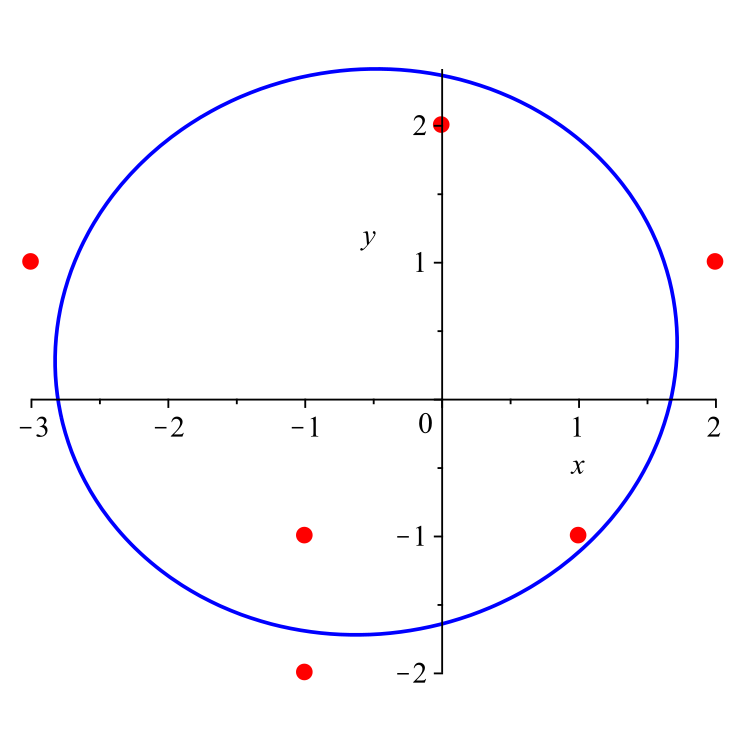
\includegraphics{ellipse_plot}}
\caption{Best fit ellipse.}
\label{F:ellipse}
\end{center}
\end{figure}

\begin{pactivity} Carl Friedrich Gauss is often credited with inventing the method of least squares. He used the method to find a best-fit ellipse which allowed him to correctly predict the orbit of the asteroid Ceres as it passed behind the sun in 1801. (Adrien-Marie Legendre appears to be the first to publish the method, though.) Here we examine the problem of fitting an ellipse to data. 

An ellipse is a quadratic equation that can be written in the form 
\begin{equation} \label{eq:ellipse} 
x^2 + By^2 + Cxy + Dx + Ey + F = 0
\end{equation}
for constants $B$, $C$, $D$, $E$, and $F$, with $B > 0$. We will find the best-fit ellipse in the least squares sense through the points 
\[(0,2), \ (2,1), \ (1, -1), \ (-1, -2), \ (-3,1), \ \text{ and } \ (-1, -1).\]
A picture of the best fit ellipse is shown in Figure \ref{F:ellipse}.

\ba
\item Find the system of linear equations that would result if the ellipse (\ref{eq:ellipse}) were to exactly pass through the given points. 

\begin{comment}

\vs

\solution If these points were to lie on an ellipse whose equation has the given form, then we have the resulting system of equations
\begin{alignat*}{7}
{0} 	&{}+{}   &{4}B 	&{}{} 		&{}		&{}{}		&{}		&{}+{}	&{2}E	&{}+{}	&{}F	&{}={} 	&0&{}  \\
{4} 	&{}+{} &{}B 	&{}+{} 	&{2}C	&{}+{}	&{2}D	&{}+{}	&{}E		&{}+{}	&{}F	&{}={} 	&0&{}  \\
{1} 	&{}+{} &{}B 	&{}-{} 	&{}C		&{}+{}	&{}D		&{}-{}	&{}E		&{}+{}	&{}F	&{}={} 	&0&{}  \\
{1} 	&{}+{} &{4}B 	&{}+{} 	&{2}C	&{}-{}	&{}D		&{}-{}	&{2}E	&{}+{}	&{}F	&{}={} 	&0&{}  \\
{9} 	&{}+{} &{}B 	&{}-{} 	&{3}C	&{}-{}	&{3}D	&{}+{}	&{}E		&{}+{}	&{}F	&{}={} 	&0&{}  \\
{1} 	&{}+{} &{}B 	&{}+{} 	&{}C		&{}-{}	&{}D		&{}-{}	&{}E		&{}+{}	&{}F	&{}={} 	&0&{.} 
\end{alignat*}

\vs

\end{comment}

\item Write the linear system from part (a) in the form $A \vx = \vb$, where the vector $\vx$ contains the unknowns in the system. Clearly identify $A$, $\vx$, and $\vb$.

\begin{comment}

\vs
 
\solution We can rewrite this as the system $A \vx = \vb$, with $A= \left[ \begin{array}{crrrc} 4&0&0&2&1\\1&2&2&1&1 \\ 1&-1&1&-1&1 \\ 4&2&-1&-2&1\\ 1&-3&-3&1&1 \\ 1&1&-1&-1&1 \end{array} \right]$, $\vx = \left[ \begin{array}{c}B\\C\\D\\E\\F \end{array} \right]$, and $\vb = \left[ \begin{array}{r} 0\\-4\\-1\\-1\\-9\\-1 \end{array} \right]$. 

\vs

\end{comment}

\item Find the least squares ellipse to this set of points. Make sure your method is clear. (Note that we are really fitting a surface of the form $f(x,y) = x^2 + By^2 + Cxy + Dx + Ey + F$ to a set of data points in the $xy$-plane. So the error is the sum of the vertical distances from the points in the $xy$-plane to the surface.)


\ea

\end{pactivity}

